\ylDisplay{Rakettmootor} % Ülesande nimi
{Jaan Kalda} % Autor
{lahtine} % Voor
{2010} % Aasta
{G 10} % Ülesande nr.
{9} % Raskustase
{
% Teema: Gaasid
\ifStatement
\begin{wrapfigure}{r}{0.45\textwidth}
	\vspace{-3ex}
	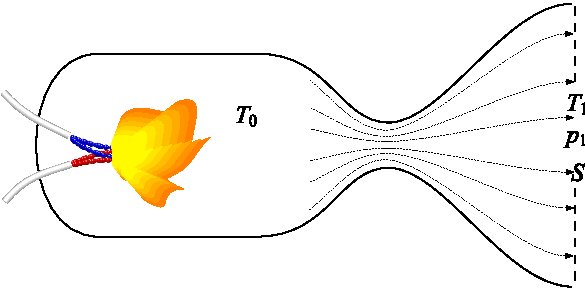
\includegraphics[width=\linewidth]{2010-lahg-10-rakettmootor}
	\vspace{-6ex}
\end{wrapfigure}
Vedelkütusel töötava rakettmootori skeem on toodud juuresoleval joonisel. Põlemiskambris moodustuvad põlemisproduktid (gaasid) omandavad kõrge rõhu ja temperatuuri. Seejärel väljuvad need adiabaatiliselt paisudes ja jahtudes läbi düüsi. Õigesti konstrueeritud düüsi korral (kaela läbimõõt vastab põlemiskiirusele ja -temperatuurile) jätkub adiabaatiline paisumine ka peale düüsikaela läbimist ning suur osa soojusenergiast muundatakse gaasijoa kineetiliseks energiaks. Leidke rakettmootori veojõud $F$ eeldusel, et (a) on teada düüsi väljundristlõike pindala $S$, temperatuur põlemiskambris $T_0$ ning gaaside temperatuur $T_1$ ja rõhk $p_1$ düüsist väljumise hetkel, kusjuures $T_0 \gg T_1$; (b) põlemiskambris on gaaside kineetiline energia tühine võrreldes soojusenergiaga; (c) atmosfäärirõhu mõju veojõule on tühine; (d) moodustuva gaasisegu ühe mooli soojusmahtuvus konstantsel ruumalal on $c_V = \frac52 R$, kus $R$ on gaasikonstant.
\fi


\ifHint
Adiabaatilisel paisumisel muutub gaasi siseenergia $c_VT_0$ osaliselt joa kineetiliseks energiaks $\mu v^2/2$. Düüsis peab kehtima energia jäävus. Seega, ajaühikus siseneval gaasihulgal on sama energia kui ajaühikus väljuval gaasil.
\fi


\ifSolution
Adiabaatilisel paisumisel muutub gaasi sisenergia $c_VT_0$ osaliselt joa kineetiliseks energiaks $\mu v^2/2$ (avaldised on siin ühe mooli gaasi jaoks); 
energia jäävuse seaduses tuleb siiski arvestada ka põlemiskambris juurde tekkivate gaaside poolt tehtavat tööd $p_0V_0$ ning
äravoolavate gaaside pidurdavat tööd $p_1V_1$, mis on olekuvõrrandi tõttu
vastavalt võrdsed $RT_0$-ga ja $RT_1$-ga. Seega, 
$$c_VT_0+RT_0=c_VT_1+RT_1+\mu v^2/2 \Rightarrow v^2=7R(T_0-T_1)/\mu.$$
Veojõud on võrdne ajaühikus eemalduva gaasijoa impulsiga,
$$F=\dot m v =(\rho_1 Sv)\cdot v=\rho_1 S v^2 = 7S\frac{R\rho_1T_1}{\mu}\left(\frac{T_0}{T_1}-1\right).$$
Arvestades gaasi olekuvõrrandit ja lähendust $T_0\gg T_1$ saame lõpptulemuseks
$$F=7Sp_1T_0/T_1.$$
\fi
}